
% Preamble
\documentclass{assignment}

% Packages
\usepackage{minted}
\usepackage{dsfont}
\usepackage{colortbl}
\usepackage[linesnumbered,ruled,longend]{algorithm2e} \usepackage[colorlinks=true,linkcolor=blue]{hyperref}


\SetKwInOut{Input}{Input} \SetKwInOut{Output}{Output} \SetKwProg{Fn}{Function}{\string:}{end} \SetKwFunction{algohw}{AlgoHw}

% Document
\begin{document}

    \maketitle

    \newpage
\begin{homeworkProblem}

\begin{enumerate}
\item Depth-First Search, is used to search or traverse tree or graph. It will explore edges out of the most recently discovered vertex $v$. Once all the edges of $v$ has been discover, it will backtrack to the vertex that $v$ is discovered. When all the vertex has been explored, the process will end. When use DFS for a graph, it will create a depth-first forest, composing several depth-first trees. Define each vertex initially white, when it is first discovered, grayed. When it is finished, such that all the adjacent list has been explore, blacked. Also use variable $time$ to timestamp for the discovering time and finishing time.


\SetKwFunction{myFunc}{DFS}
\SetKwFunction{my}{DFS-VISIT}
  \begin{algorithm}[H]
\Input{graph $G = (V, E)$}
\Output{depth-first forest} \BlankLine
\Fn{\myFunc{G}}{
\For {each vertex $u \in G.V$} {
	$u.color \leftarrow WHITE$ \\
	$u. \pi \leftarrow NULL$ \\
}
$time\leftarrow$  0 \\
\For {each vertex $u \in G.V$} {
\If{u.color == WHITE} 
{	\my{G, u}\\
	}
	}
	}
\Fn{\my{G,u}} {
	time $\leftarrow$ time + 1 \\
	$u.d \leftarrow time$ \\
	$u.color \leftarrow GRAY$ \\
	\For {each v $\in$ G.adj[u]} {
		\If{v.color == WHITE} {
		v.$\pi = u$ \\
			\my{G,  v} \\		
		}
	}
	u.color $\leftarrow$ BLACK \\
	time $\leftarrow$ time + 1\\
	u.f $\leftarrow$ time \\
}	
	
	
\caption{DFS} \end{algorithm}


\item Topological sorting is for directed acyclic graph. A linear ordering of vertices such that if a directed edge $u \leftarrow v$, then $u$ should be before $v$ in the ordering. It will print a vertex before its adjacent vertices while DFS will print a vertex then call DFS for its adjacency vertices. It could be easily realized through DFS. Because a vertex with smaller finish time should be deeper in the graph, so put each finished vertex at the begin of the result sorting list then could get a topological sorting list. 

\SetKwFunction{myFunc}{DFS}
\SetKwFunction{my}{DFS-VISIT}
  \begin{algorithm}[H]
\Input{graph $G = (V, E)$}
\Output{topological sorted list} \BlankLine
\myFunc{G} to compute each vertex's finish time \\
as each vertex is finished, insert it into the front of the result $list$ \\
\KwRet{list}

	
\caption{Topological Sorting} \end{algorithm}
\item Given a DAG, because Hamiltonian path is a path that includes every vertex, perform a topological sorting and check whether successive vertices are connect in the graph. These edges form a directed Hamiltonian path. The DFS algorithm is modified a bit, only result that would be used for finding Hamiltonian path is kept.


\SetKwFunction{topo}{DFS}
\SetKwFunction{topolo}{DFS-VISIT}
  \begin{algorithm}[H]
\Input{A DAG graph $G = (V, E)$}
\Output{whether $G$ contains a Hamiltonian path} \BlankLine
\Fn{\topo{G}}{
\For {each vertex $u \in G.V$} {
	$u.color \leftarrow WHITE$ \\
	$u. \pi \leftarrow NULL$ \\
}
$list \leftarrow []$ \\
\For {each vertex $u \in G.V$} {
\If{u.color == WHITE} 
{	\topolo{G, u, list}\\
	}
	}
	\KwRet{list}
	}
\Fn{\topolo{G, u, list}} {
	$u.color \leftarrow GRAY$ \\
	\For {each v $\in$ G.adj[u]} {
		\If{v.color == WHITE} {
		v.$\pi = u$ \\
			\topolo{G, v, list} \\		
		}
	}
	u.color $\leftarrow$ BLACK \\
	insert $u$ at the front of $list$\\
}	
$result\leftarrow \topo{G}$ \\
\For{i $\leftarrow$ 0 \KwTo $result.size - 1$} {
	\If {result[i] do not connect with result[i+1]} {
	\KwRet{False}}
	
}
\KwRet{True}

	
\caption{Hamiltonian Path in DAG} \end{algorithm}

\item Assume the graph $G = (V, E)$. Because in function \topo , first initialize all the vertex (line 2-5), which is in $\Theta(V)$, then the loop on line 7-11 will be performed in $\Theta(V)$ if exclude the time for \topolo . Using aggregate analysis, because each vertex will be coloured after discovered, so each vertex is discovered for only one time. \topolo is called one time for each $v \in V$. For each $v$, its adjacent vertex $u$ will be invoked into this turn if it is white. So during each \topolo{G, u}, the loop on line 16-22 is executed $|Adj[v]|$ times. As we have $$\sum_{v\in V}|Adj[v]| = \Theta(E),$$ the total time for line 16-22 is $\Theta(E)$. Then the running time for \topo is $\Theta(V + E)$.

 As we have $V$ elements in $result$, the loop in line 26-30 will be executed in $\mathcal{O}(V)$. So its complexity is $\mathcal{O}(V+E)$.
 \item It belongs to NP-class. 

\end{enumerate}
\end{homeworkProblem}
	% Q1
    \begin{homeworkProblem}
    \begin{enumerate}
\item No. To prove a function $f(n)$ is polynomial bounded, it is same to prove  $log(f(n))$ is bounded by $\mathcal{O}(log(n^k))$, such that there exist constant $c, n_0, k$ such that for any $n > n_0$, $log(f(n)) \leq cklogn$.  

First prove $log(n!) = \Theta(n\cdot logn)$ 
\begin{align*}
log(n!) &= log(1) + log(2) +... log(n) \\
 &\leq log(n)+log(n)+...log(n) = nlog(n) \\
 log(n!) &\geq log(n/2) + log(n/2 + 1) + … +log(n-1) + log(n) \\ &\geq log(n/2)+ log(n/2) + … + log(n/2) = (n/2)log(n/2)  \\ &= (n/2)(logn + log(1/2))\\ &= (n/2)logn - n/2
\geq 1/4(nlogn).
\end{align*}
Then $$log(\lceil logn \rceil !) = \Theta (\lceil logn \rceil \cdot log ( \lceil logn \rceil )).$$

    Also it is easy to get $\lceil logn \rceil = \Theta(logn).$ So we have 
    $$log(\lceil logn \rceil !) = \Theta ( logn  \cdot log ( logn )).$$
   Then prove   $\lceil logn \rceil !$ is not bounded by a polynomial by contradiction. Assume it is bounded by a polynomial, then   $log (\lceil logn \rceil !) = \mathcal{O}(logn ),$ such that $logn  \cdot log ( logn )= \mathcal{O}(logn )$, which is obviously wrong. So  $\lceil logn \rceil !$ is not bounded by a polynomial. 
    \item Yes. When $n>1$, $log^*n = 1 + log^*logn$. $log^*n$ is the number of log need to be applied to n to reach the fixed value 1. \\
    When $n>1$, it is easy to obtain $logn < n -1$ as $\frac{d(logn)}{dn} = \frac{1}{n} < 1 = \frac{d(n-1)}{dn}$. So  $$loglog^*n = log(1 + log^*logn) < log^*logn.$$
    \item The minimized number of weighing could be 2.     
    
     \begin{algorithm}[H]
\Input{eight balls with similar size $a1, a2, ..., a8$, one of which is lighter}
\Output{the lighter ball $a0$} \BlankLine
Divide the balls into three groups $(a1, a2, a3), (a4,a5,a6), (a7, a8)$ \\
\textbf{First Weighing:} compare the weight of $(a1,a2,a3)$ with $(a4,a5,a6)$ \\
\uIf {$(a1,a2,a3).weight == (a4,a5,a6).weight$} {
\textbf{Second Weighing:} compare the weight of $a7$ and $a8$ \\
$a0 \leftarrow min(a7.weight, a8.weight)$\\
} \tcc{assume $(a1,a2,a3)$ is lighter without losing generality}
\Else{ 
\textbf{Second Weighing:} compare the weight of $a1$ and $a2$ \\
\uIf{$a1.weight == a2.weight$} {$a0 \leftarrow a3$}
\Else {$a0 \leftarrow min(a1.weight, a2.weight)$}
}
\caption{Find a lighter ball} \end{algorithm}
    \end{enumerate}
    
    \end{homeworkProblem}
    
    \begin{homeworkProblem}
    Rubik's Cube is made up of 26 mini cubes and each of them is called cubie. Turn the cube to make each face (a side of the cube) to have the same color. The center, edge and corner cubie refers to a cubie with one sticker, two stickers and three stickers respectively. Twist if a 90 or 180 degree turn of one of the six face,  use F, B, U, D, L, and R designate 90-degree turns of the front, back, up, down, left, and right faces, respectively. Add ' (such that F') is a 90-degree counterclockwise “prime” twist, and add 2 (such that F2) is a 180-degree twist. 
\begin{enumerate}
\item the beginner's method\cite{cube}. The whole step is shown in the Figure \ref{fig:beg}. It divides the cube into layers and solve each layer without messing up the pieces that already in place. 

\begin{figure}[!ht]
\centering
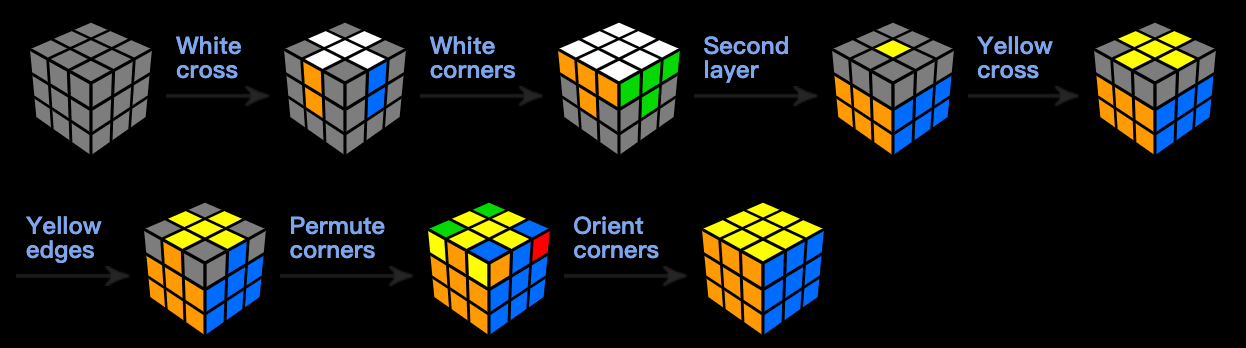
\includegraphics[scale=0.6]{cube1.png}
\caption{Step by step solution for beginner's method}
\label{fig:beg}
\end{figure}
\begin{enumerate}
\item[a.] First layer: choose white (or any other color) to get white cross, then get white corners to finish the first layer. An algorithm that would always be valid to bring a white corner piece to the top layer without break the solved pieces is R'D'RD.
\item[b.] Second layer: put the top layer face down now. Two algorithms to make the front-up edge to the right-front or left-front positions, called right algorithm (URU'R'U'F'UF) and left algorithm (U'L'ULUFU'F').  
\item[c.] Last layer: make a yellow cross first (FRUR'U'F') then for yellow edges (RUR'URU2R'U to switch the front and left yellow edges). Premutation for the last layer (URU'L'UR'U'L) then do the orientation.  
\end{enumerate}
\item CFOP method. The advanced Fridrich (CFOP) method still divides the problem into different layers, and apply different algorithm for each step shown in Figure \ref{fig:cfop}.

\begin{figure}[!ht]
\centering
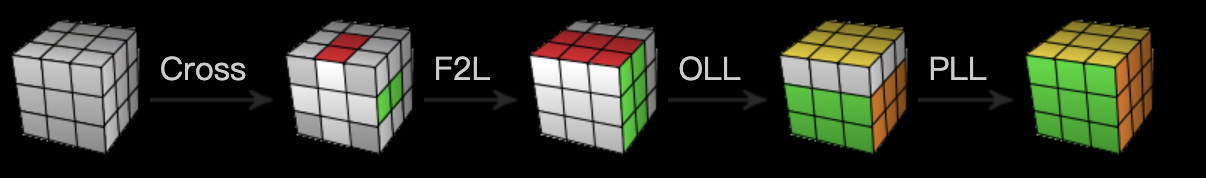
\includegraphics[scale=0.6]{cube2.png}
\caption{Steps of CFOP method}
\label{fig:cfop}
\end{figure}
\begin{enumerate}
\item[a.] Complete the white cross (or choose any other color), but need to foresee 7 steps to succeed, 

\item[b.] Solve the first two layers (F2L) through pairing white corner and second layer edge pieces. It could be done intuitively or memorize different algorithm for different situations. 
\item[c.] Orienting the last layer (OLL). Solve the yellow face without matching the side colors. 
\item[d.] Permutate the last layer (PLL).  
\end{enumerate}

\end{enumerate}    

\bibliographystyle{unsrt}
\bibliography{sample}
    
    \end{homeworkProblem}
        \begin{homeworkProblem}
        To prove a problem is in $\mathcal{NP}$, show that a certificate could be used with a verifier running in deterministic polynomial time to recognize the given problem. 
        \begin{enumerate}
        \item Certificate: a simple path $y$. Verifier: traverse the vertices to see whether $y$ is a simple path, running in $\mathcal{O}(|V|)$.
        \item Certificate: a factor $y$ of the given integer $n$. Verifier: do $n \% y$, easily implement in polynomial time.
        \item Certificate: a vertex cover of size $k$. Verifier: For each edge $e=(u,v) \in E$, check whether either $u$ or $v$ is in the vertex cover, running in $\mathcal{O}(|E|\cdot k )$.
          
        \end{enumerate}
\end{homeworkProblem}
    
    
    
    %Q3
    \begin{homeworkProblem}
    
    It is not sufficient to prove that PRIMES is in $\mathcal{P}$. It is obvious that by dividing $n$ using incremented integers, the process could be stopped when the integer is larger than $\sqrt{n}$.
    
         \begin{algorithm}[H]
\Input{integer $n$}
\Output{whether $n$ is a prime number} \BlankLine
$i \leftarrow 2$  \\
\While{i $\leq \sqrt{n}$} {
\If {n $\%$ i == 0} {\KwRet {True}}
$i \leftarrow i + 1$ \\
 }
\KwRet{False}
\caption{trivial division for PRIMES} \end{algorithm}
 The loop will be executed for at most $\sqrt{n}$ times,
    \textbf{Prime Number Theorem:} $\pi (N) \sim  \frac{N}{log(N)}$, where $\pi (N)$ is the function counting the prime number smaller or less than $N$ and $log(N)$ is the natural logarithm of $N$. 
    \end{homeworkProblem}
    




\end{document}
